\chapter{What is the "FED Put" and how can it be explained?}
\section{The FED Put}
The FED Put in general refers to (or, moreover, to the expectation of) a strong accommodating monetary policy by the Federal Reserve (FED), by which, in case of a sharp decline in asset prices, the FED is expected by the market (its investors) to intervene. The term is coined from the concept of a "put option" in asset markets, which gives the buyer the option to sell at a predetermined price. Thus, the FED would protect an investor from the decline in the value of an asset.\footnote{\url{https://corporatefinanceinstitute. com/resources/economics/FED-Put/}}

Central banks have gained credibility ever since the mid-1980s by keeping inflation low (\cite{hall_is_2011} 2011). The related term "Greenspan Put" is often used to describe the monetary policy under former Federal Reserve Chairman Alan Greenspan to intervene in financial markets in order to prevent significant declines or disruptions. 

While some argue that market interventions are necessary to prevent financial crises (like the Dot-com bubble burst in 2001 or Lehman Brothers in 2008), others believe that these interventions distort the market and create unnecessary moral hazard (\cite{cieslak_economics_2021},  2021),  meaning that investors are willing to take on excessive risks because they believe that the FED will always come to rescue them arguing that such "too big to fail” beliefs or mentality can lead to financial crises in the long run.

\section{Stock Returns over the FOMC Cycle}

Diving further into dynamics like the FED Put,  \cite{cieslak_stock_2019} (2019) focuses on a FOMC cycle specific pattern of the equity premium since 1994. 
The stock returns exhibit a distinct,  statistically significant pattern over the FOMC cycle.  Notably,  it primarily accrues in even weeks of the FOMC cycle time (for a graphical explanation of the FOMC cycle, see figure~\ref{cies19_fig2} on page~\pageref{cies19_fig2}). For calculation of stock excess returns the authors use research portfolio data provided by Kenneth R. French for convenience\footnote{\url{https://mba.tuck.dartmouth.edu/pages/faculty/ken.french/data_library.html\#research}}.

\begin{figure}[h]
    \centering
    \label{cies19_fig1}
    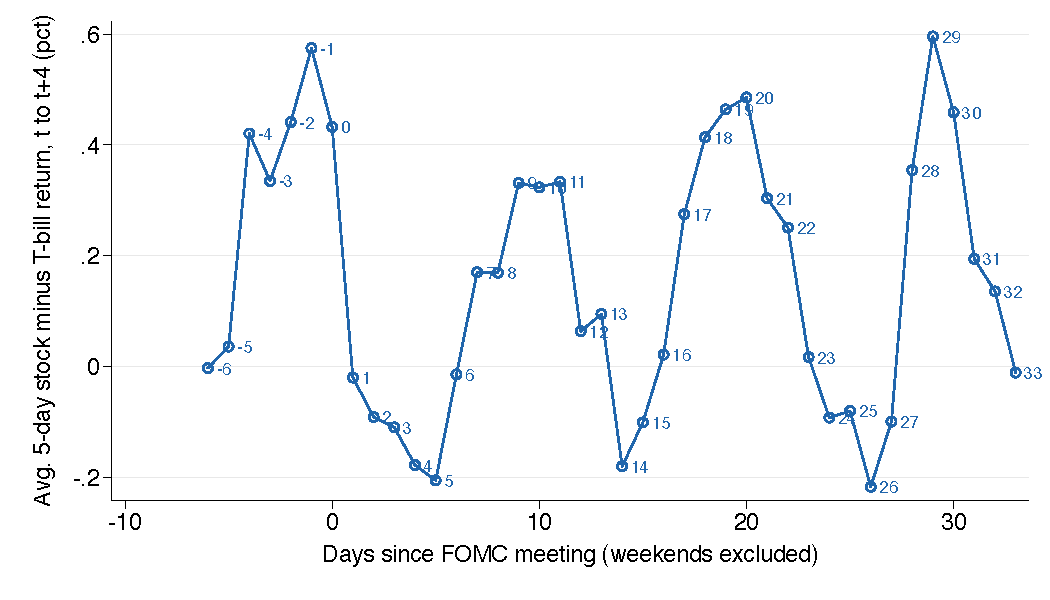
\includegraphics[width=0.9\textwidth]{figures/cies19/fig1}
    \caption{Average 5-day stock excess returns over FOMC cycle time (pct) (\cite{cieslak_stock_2019}, 2019) }
\end{figure}

The authors present three different trading strategies (A, B, and C) that demonstrate the influence of the FOMC cycle on stock market returns.  Of particular note is Strategy A, which involves exclusively holding stocks during even FOMC cycle weeks (and investing in a "risk-free" rate during odd FOMC cycle weeks). This strategy demonstrates that the average annual return more than doubles compared to holding for example an ETF throughout the entire FOMC cycle.  Conversly, the authors find that holding an ETF during uneven FOMC weeks (compared to a "risk-free" rate) resulted in financial losses over the examined period from 1994 to 2016.  This results have also been covered by the media.\footnote{\url{https://www.economist.com/finance-and-economics/2016/09/03/the-long-arm-of-the-FED}}

\begin{figure}[h]
    \centering
     \label{FED_long_arm}
    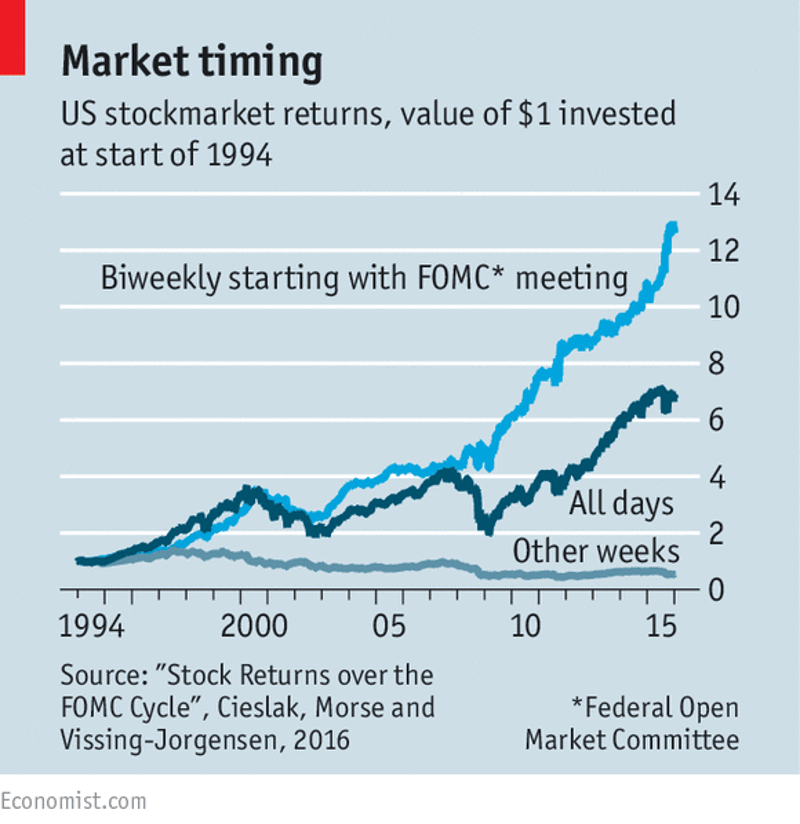
\includegraphics[width=0.6\textwidth]{figures/20160903_FNC453.png}
    \caption{\cite{noauthor_long_2016}}
\end{figure}

The authors extend their analysis to explore whether the FOMC cycle return pattern extends beyond the United States, potentially influenced by movements of the dollar currency. To investigate this, they use ETFs containing globally diversified stocks. To establish causality, the authors compare FOMC cycles with other macroeconomic news calendars (e.g., Bloomberg macroeconomic news), dispelling the notion that macroeconomic news significantly correlates with FOMC cycle calendars. They also provide evidence that the release of quarterly firm profits does not substantially account for the observed equity premium patterns over the FOMC cycle.

The authors examine a causal link between the FED's policy actions and the behavior of the stock market by analyzing in the Federal Fund target changes between meetings,  FED funds futures and internal meetings of the Board of Governors. They propose that the FED's anticipated accommodative policies have a substantial impact on the stock market, resulting in a increase of the overall equity premium.  Additionally, they contend that there is evidence of informal communication channels between FED officials, the media, and the financial sector, which serve as a means for disseminating information about monetary policy to the market.

\begin{figure}[h]
    \centering
    \label{cies19_fig3A}
    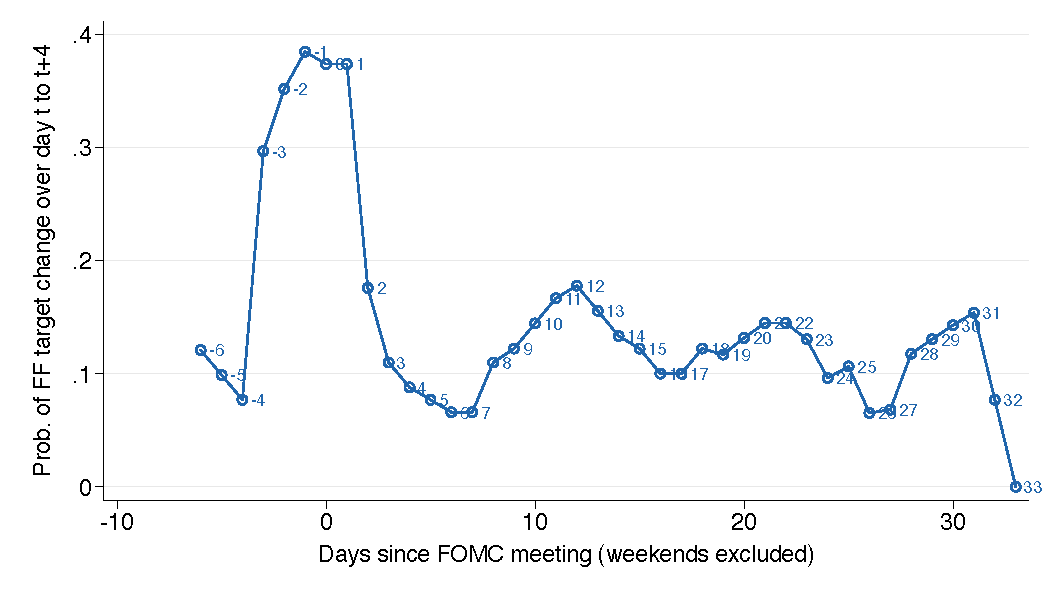
\includegraphics[width=0.9\textwidth]{figures/cies19/fig3A}
    \caption{Probability of FFR target changes within FOMC cycle time (\cite{cieslak_stock_2019}, 2019) }
\end{figure}

\pagebreak

\section{The Economics of the FED Put}
\cite{cieslak_economics_2021} (2021) further attempts to study the economics of the relationship between FED policy and the stock market. The authors compare the stock market's predictive power to other economic indicators to forecast changes in the Federal Funds Rate (FFR) using textual analysis from former FOMC meeting transcripts.\footnote{\url{https://www.federalreserve.gov/monetarypolicy/fomc_historical.htm}} Their findings affirm that the FED indeed pays a lot of attention to the stock market during market downturns.

\begin{figure}[h]
    \centering
        \label{cies21_fig5}
    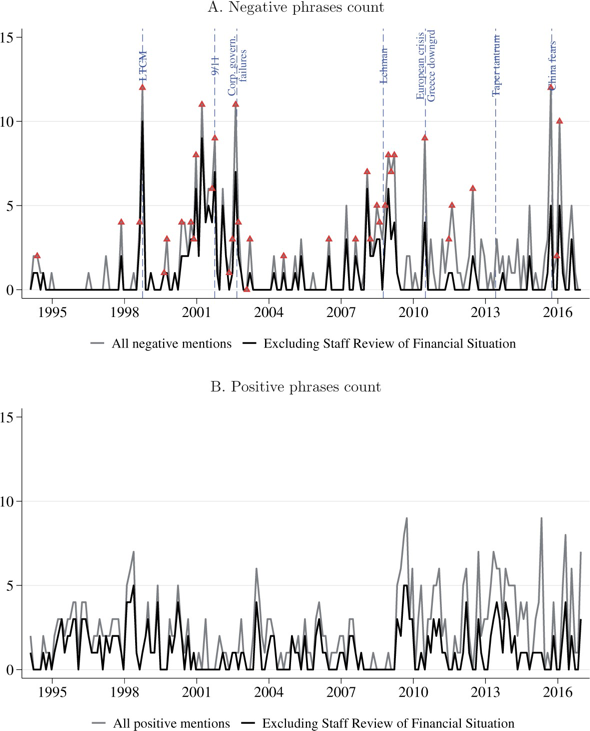
\includegraphics[width=0.9\textwidth]{figures/cies21/Figure5}
    \caption{Negative and positive phrases of the stock market count (\cite{cieslak_economics_2021}, 2021)}
\end{figure}

They argue that the FED Put is fueled by the Federal Reserve's concerns about wealth effects on consumption. Conversely, strong stock market performance corresponds to updates of the FED’s internal growth projections. Empirical evidence substantiates their claims, as multiple regressions of changes in the FFR demonstrate that the stock market explains a higher proportion of the variance (R-squared) compared to other macroeconomic indicators. Importantly, this relationship appears to be less pronounced before the 1990s period.  

During the third European Central Bank (ECB) annual research conference\footcite{european_central_bank_third_2018} in 2018, valuable comments on the econometric approach by the authors were made by the discussant, Emmanuel Moench, the former head of research at the Bundesbank. Moench suggests that the correlation between stock excess returns and the FFR is heavily influenced by two specific FOMC meetings (during financial crises like the dot-com bubble burst in 2001 and the 2008 financial crisis). Furthermore, he recommended incorporating additional covariates, including consumer confidence news and credit spreads, into the regression models to enhance their explanatory power. Moench sees the stock market as one of several co-factors influencing Federal Reserve policy (presumably over the updates of the FED's growth projections as stated by the authors), rather than a dominant driver of the FED's policy.

